\documentclass[11pt,letterpaper]{article}
\usepackage[T1]{fontenc}
\usepackage[utf8]{inputenc}
\usepackage{lmodern}
\usepackage[margin=1in,headheight=14pt]{geometry}
\usepackage{amsmath,amssymb,amsthm,mathtools}
\usepackage{microtype,booktabs,longtable,array,enumitem}
\usepackage{graphicx,tikz}
\usetikzlibrary{arrows.meta,positioning}
\usepackage[numbers,sort&compress]{natbib}
\usepackage{xurl}
\usepackage[hidelinks]{hyperref}
\hypersetup{pdftitle={Closure-Aware Cut Certificates and First-Hit Factorization},
 pdfauthor={ProveIt research contribution prepared with ChatGPT},
 pdfsubject={Sharp homology budgets and exact unknot recognition}}
\usepackage{fancyhdr}
\usepackage{listings}
\pagestyle{fancy}\fancyhf{}
\fancyhead[L]{\small Closure-aware cut certificates}
\fancyhead[R]{\small ProveIt research contribution}
\fancyfoot[C]{\thepage}
\setlength{\parskip}{4pt}
\setlength{\parindent}{1.2em}
\setlist{itemsep=3pt,topsep=5pt}
\lstset{basicstyle=\small\ttfamily,breaklines=true,columns=fullflexible,keepspaces=true,
 frame=single,framerule=0.3pt,xleftmargin=2pt,xrightmargin=2pt}
\newtheorem{theorem}{Theorem}[section]
\newtheorem{lemma}[theorem]{Lemma}
\newtheorem{proposition}[theorem]{Proposition}
\newtheorem{corollary}[theorem]{Corollary}
\theoremstyle{definition}\newtheorem{definition}[theorem]{Definition}
\newtheorem{example}[theorem]{Example}
\theoremstyle{remark}\newtheorem{remark}[theorem]{Remark}
\newcommand{\F}{\mathbb F_2}
\newcommand{\rk}{\operatorname{rank}}
\newcommand{\im}{\operatorname{im}}
\newcommand{\Kh}{\widetilde{\operatorname{Kh}}}
\newcommand{\poly}{\operatorname{poly}}
\newcommand{\code}[1]{\texttt{#1}}
\newcommand{\qpoly}{\exp\!\bigl(O(\log^2(n+2))\bigr)}
\newcommand{\cutlb}{\beta_{\mathrm{cut}}}
\title{\textbf{Closure-Aware Cut Certificates\protect\\and First-Hit Factorization}\\[5pt]
\large Sharp homology budgets and terminal dimension bounds\protect\\
for exact unknot recognition}
\author{A research contribution prepared for the ProveIt project\\
\small Mathematical analysis and reference implementation prepared with ChatGPT}
\date{8 October 2026}
\begin{document}
\maketitle
\begin{abstract}
We develop an exact, decision-oriented refinement of the graded and corridor
transfer methods in ProveIt's unknot-recognition project. A transferred
cobordism differential is a finite typed path sum. Factoring that sum at the
\emph{first} visit to an arbitrary vertex separator gives an exact product
$D=BA$, without an antichain hypothesis or commuting coefficients. After a
fixed verified closure, the sum of the separator's vector-space dimensions
bounds the differential rank. We combine these bounds with the adjacent-degree
constraints imposed by $d^2=0$. The resulting capacitated path-matching problem
has a simple optimal greedy solution and yields the strongest homology lower
bound available from those dimensions and rank caps alone.

For a certified reduced knot complex, a lower bound greater than one rejects
the unknot without evaluating the remaining transferred coefficients.
Otherwise the closed critical dimension is at most twice the optimized rank
budget plus one. Exact rank computation through the cut factors avoids
materializing a dense terminal differential. We prove the factorization,
the sharp budget theorem, the decision dichotomy, and an explicit separation
from both endpoint-propagation directions on a valid algebraic family.

The accompanying standard-library Python package passes 36 unit tests and an
audit of 80 small braid diagrams in 160 matching configurations, covering
1,070 transferred maps. In seven-round paired experiments, min-cut discovery
is overhead on the small knot examples; the largest constructed bottleneck
example gives a $4.80\times$ exact-rank-stage improvement over forward
propagation. This is not an end-to-end production speedup. The results provide
an optional research kernel, independently replayable small-input certificates,
and precise conditional quasi-polynomial bounds. They do not establish a
quasi-polynomial bound for arbitrary knot diagrams or implement the missing
geometric construction and production closure adapter.
\end{abstract}
\vspace{4pt}
\noindent\textbf{Status.} Complete proofs for the stated algebraic results;
executed reference-code validation; proposed, not performed, integration into
the maintained recognizer. No formal proof-assistant verification is claimed.
\newpage
\tableofcontents
\newpage

\section{Research target, provenance, and contribution}
\subsection{What is being improved}
The practical question is not whether a full homology computation can be
expressed as a finite calculation. It is whether the information needed for a
\emph{rank-one decision} can be extracted without creating every intermediate
matrix entry or expanding every terminal generator. An exact recognition
algorithm may reject as soon as certified homology dimension exceeds one;
it need not compute that dimension in full.

The maintained project overview distinguishes the existing exact recognizers
from a proved general quasi-polynomial implementation \cite{repo}.
Two especially relevant maintained articles supply graded perturbation
transfer and survivor-corridor pruning with forward or reverse propagation
\cite{repograded,repocorridor}. We build on their path-sum viewpoint rather than
reintroducing local cancellation, visible connected-sum decomposition, or
an invariant filter as a new recognition algorithm.

The specific additional question addressed here is:
\begin{quote}
Can a small \emph{internal} interface control an entire transferred map even
when both terminal sets are large, and can that interface certify enough
homology to make the remaining exact computation unnecessary?
\end{quote}
The answer is yes for explicit acyclic transfer graphs, with closure-dependent
capacities and a carefully stated knot-complex contract. The hard unresolved
question is how cheaply such graphs and useful interfaces can be produced
for arbitrary classical knot diagrams.

\subsection{Repository snapshot and review scope}
The branch reference observed during this work was
\begin{center}\small
\code{bc5b913850f78155ccfddd808d4b11517dca252d}.
\end{center}
Its recorded commit time was 8 October 2026, 16:46:30 UTC. The reviewed
full texts were the project overview and the maintained graded-transfer and
corridor-transfer articles. Their Git blob identifiers are retained in
\code{PROVENANCE.json}. The corridor article's blob was additionally checked
at the pinned commit. Directory listings and targeted repository searches
were used to locate related work.

This is a source review, not a full checkout or a full upstream regression
run. The supplied code is an independent research package: it neither vendors
nor modifies the maintained scanner. In particular, the 36 tests reported
here are this package's tests, not the maintained project's test count.
Repository search was not an exhaustive novelty search. The elementary
network and linear-algebra ingredients are not claimed as newly discovered
mathematics; the contribution is their precise combination, specialization,
proof obligations, and tested decision-oriented use at this transfer boundary.

\subsection{External status of the asymptotic target}
Oxford publicly announced Lackenby's quasi-polynomial unknot-recognition
result in 2021 \cite{oxford2021}. His July 2026 hierarchy preprint gives a
new algorithmic approach; Section 9 explicitly distinguishes a bound on step
counts from a bound on the cost of all individual steps \cite{lackenby2026}.
An announcement of a general theorem, the specifications in that preprint,
and the guarantees of this project's executable recognizer are different
claims. Our homological construction does not fill in those hierarchy
routines, and no conclusion about their eventual complexity is inferred
from our experiments.

\subsection{Main statements and their logical order}
The core results form a short dependency chain. First-hit factorization
(Theorem~\ref{thm:firsthit}) is purely categorical. Closure converts it into
rank caps (Theorem~\ref{thm:capacity}). The optimal rank-budget theorem
(Theorem~\ref{thm:budget}) turns those caps into a sharp homology lower bound.
The rank-one decision dichotomy (Theorem~\ref{thm:dichotomy}) then either
rejects or bounds the size of the remaining closed terminal problem.
Finally, Theorem~\ref{thm:complexity} states the costs that must be bounded
to obtain a quasi-polynomial recognition result on a specified input class.

The finite examples test implementations of these statements. They do not
prove the geometric hypotheses of the complexity theorem. Conversely,
negative timings on small diagrams do not invalidate the algebraic
factorization or its asymptotic separation from endpoint propagation.

\section{Exact input model and the transfer boundary}
\subsection{The knot-complex contract}
Let $K$ be a one-component classical knot and let $C(K)$ be its finite reduced
Khovanov cochain complex over $\F$. We normalize the marked crossingless
unknot to a single generator in bidegree $(0,0)$. Thus a verified chain
homotopy equivalent complex $R$ has
\[
\dim_{\F}H(R)=\dim_{\F}\Kh(K;\F).
\]
The normalized degree matters for graded certificates, but total rank does
not depend on an overall grading shift.

Kronheimer--Mrowka's detection theorem gives the rank-one criterion
\cite{km2011}. For the binary version used here, universal coefficients imply
that rational reduced rank is at most binary reduced dimension. The rational
reduced theory is nonzero for a knot: its Euler polynomial is the normalized
Jones polynomial, which takes value one at one. Hence binary dimension one
forces rational rank one and therefore the unknot; the unknot itself has
binary dimension one. A verified binary dimension exceeding one excludes
the unknot simply by invariance. No assertion about detection by the Jones
polynomial alone is used.

A graph with user-supplied dimensions is \emph{not} a knot certificate.
Any topological conclusion below requires that the graph describe an exact
transferred differential for the specified reduced knot complex, or that a
separate verified chain equivalence establish this fact. This input-origin
condition is as important as the subsequent algebra.

\subsection{Typed finite path sums}
Let $\mathcal A$ be an additive category whose morphism groups are
$\F$-vector spaces and whose composition is bilinear. A finite directed
acyclic graph $G=(V,E)$ has an object $X_v$ at each vertex and a morphism
$f_e:X_u\to X_v$ on each edge $e=(u,v)$. Let $S,T\subseteq V$ be disjoint
source and target sets. Sources have no incoming edges, and targets have no
outgoing edges. Vertices unrelated to a source--target path may be retained;
pruning them is optional.

For a path $\pi=(v_0,\ldots,v_m)$ write
\[
 f_\pi=f_{v_{m-1}v_m}\circ\cdots\circ f_{v_0v_1}.
\]
A length-zero path contributes the identity. The path-sum transfer is
\begin{equation}
D_{ts}=\sum_{\pi:s\leadsto t}f_\pi,
\qquad D:\bigoplus_{s\in S}X_s\longrightarrow\bigoplus_{t\in T}X_t.
\label{eq:pathsum}
\end{equation}
Acyclicity makes the sum finite. Distinct paths can cancel in characteristic
two; nonzero individual morphisms can have zero composite. Reachability is
therefore an upper approximation to algebraic support, not an exact test of
nonzero entries.

The abstract theorem also works over another coefficient ring with an
additive category and the appropriate signed transfer graph. The shipped
integer encodings use XOR addition and so implement characteristic two only.

\subsection{Why this graph appears in cancellation}
Local cancellation in Khovanov computations and algebraic Morse theory are
established constructions \cite{barnatan2007,kozlov2005,skoldberg2018}.
The particular production setting reviewed here splits $d=d_0+\delta$,
contracts the scalar part $d_0$, and obtains
\begin{equation}
D=P\delta(1+H\delta)^{-1}I
 =\sum_{r\geq0}P\delta(H\delta)^rI.
\label{eq:hpl}
\end{equation}
Here $I,P,H$ are the actual inclusion, projection, and contracting homotopy,
not merely the ranks of the scalar matrices. Nilpotence follows from a
verified acyclic order. In the maintained graded implementation that order
uses the strictly increasing quantum weight of radical arrows
\cite{repograded}. In our closed reference implementation it is supplied by
an explicitly checked acyclic Morse matching.

The degree-$h$ transfer graph has copies of degree-$h$ and degree-$(h+1)$
objects, the terminal survivors, and edges for $I,\delta,H,P$.
The $H$ arrows run back by one cohomological degree. Consecutive factors in
\eqref{eq:hpl} give exactly the directed source--target paths. The resulting
path sum is a differential on the survivors because it comes from a chain
contraction. An arbitrary path-sum matrix, in isolation, need not form a
complex with its neighboring matrices.

Our closed cube tests use a simpler special case. Chosen scalar differential
entries form disjoint identity pairs. Their arrows are reversed, all other
differential arrows remain forward, and the whole directed graph is checked
for cycles. The elementary two-term contractions and their finite perturbation
produce the Morse differential. In this closed Morse model, unlike the
production scalar/radical split, $\delta$ may itself contain scalar entries;
acyclicity is the termination condition. All signs disappear over $\F$. This
validation does not assume that a closed binary differential strictly raises
the normalized quantum degree; in fact it preserves that degree.

\section{First-hit factorization through an arbitrary separator}
\begin{definition}
A vertex separator $Q\subseteq V$ meets every directed path from $S$ to $T$.
It may contain terminals, and it need not be an antichain. For $q\in Q$ define
\[
 A_{qs}=\sum_{\substack{\pi:s\leadsto q\\
                  q\text{ is the first vertex of }Q\text{ on }\pi}}f_\pi,
 \qquad
 B_{tq}=\sum_{\rho:q\leadsto t} f_\rho.
\]
The suffix sum is unrestricted: it may pass through other vertices of $Q$.
If $s\in Q$, its only first-hit prefix is the length-zero path at $s$.
\end{definition}

\begin{theorem}[First-hit separator factorization]\label{thm:firsthit}
In the typed acyclic setting of \eqref{eq:pathsum}, every vertex separator
$Q$ gives
\begin{equation}
D=BA:\bigoplus_{s\in S}X_s\xrightarrow{A}
       \bigoplus_{q\in Q}X_q\xrightarrow{B}
       \bigoplus_{t\in T}X_t.
\label{eq:factor}
\end{equation}
No invertibility, commutativity, generic-rank, or antichain hypothesis is
required. The factorization is valid even when the final sum vanishes.
\end{theorem}
\begin{proof}
Every source--target path meets $Q$ and has a unique first such vertex $q$.
Split it there. Its prefix is one of the paths contributing to $A_{qs}$,
and its suffix contributes to $B_{tq}$. Conversely, concatenate any allowed
prefix to $q$ with any suffix from $q$ to $t$. A repeated vertex other than
$q$ would form a directed cycle, so the concatenation is a path. Its first
visit to $Q$ is $q$. We have a bijection between original paths and the pairs
of paths indexing the matrix product $BA$. Ordered composition of their
morphisms gives the original path product. Bilinearity now proves each
matrix entry of \eqref{eq:factor}. Cancellations take place identically on
both sides of the equality.
\end{proof}

\subsection{A tempting but incorrect variant}
It is not valid to use unrestricted prefixes and unrestricted suffixes for
an arbitrary separator. In the chain
\[
s\longrightarrow q_1\longrightarrow q_2\longrightarrow t
\]
put every edge coefficient equal to one and take $Q=\{q_1,q_2\}$.
The original transfer is one. An unrestricted split at either cut vertex
counts the same path twice, giving zero over $\F$. Thus an implementation
that quietly treats every minimum vertex cut as an antichain can compute a
wrong differential. The issue can occur for a minimum cut, not just a
redundant separator. Add edges $s\to q_2$ and $q_1\to t$ to the displayed
chain, give $s,t$ capacity three and $q_1,q_2$ capacity one. Then
$\{q_1,q_2\}$ is the unique minimum vertex separator, of capacity two.
There are three source--target paths, so the actual binary transfer is one;
unrestricted splitting counts the two-cut path twice and again gives zero.
First-hit prefixes remove the ambiguity without placing extra restrictions
on the optimizer.

The same example explains why the suffixes must remain unrestricted. If
both prefixes and suffixes were required to avoid other cut vertices, the
unique original path would disappear. The two asymmetric rules are a pair:
first-hit on the left, unrestricted on the right.

\subsection{An exact implementation and its costs}
Let $a=|S|$, $b=|T|$, and $r=|Q|$. For each $q$, compute its prefix row by
reverse propagation from $q$, stopping propagation at every other vertex of
$Q$. Contributions that reach another cut source are explicitly excluded
from the row. Compute its suffix column by ordinary forward propagation
from $q$, without stopping at later cut vertices.

For an edge $u\xrightarrow{f}v$, reverse propagation of a current suffix
$g:v\to q$ forms $g\circ f$. Forward propagation of $g:q\to u$ forms
$f\circ g$. Exchanging those products is wrong in a typed category, even
if a particular dot-ring test happens to commute. The matrix-category tests
therefore use rectangular noncommuting binary matrices.

\begin{proposition}[Factor construction bound]\label{prop:factorcost}
After topological ordering, the factors can be computed in
$O(r(|V|+|E|))$ coefficient/control operations, storing
$O(|V|+|E|+r(a+b))$ coefficients and graph entries. This bound includes
visits to vertices whose current coefficient is zero. The reference
implementation's heap-based topological sort adds
$O(|E|+|V|\log(|V|+2))$ index operations.
\end{proposition}
\begin{proof}
There are two propagations per cut vertex. Each visits every vertex once
and attempts at most one composition and addition per edge. Working values
are reused between roots. The permanent prefix and suffix arrays have
$ra$ and $br$ entries. Standard adjacency construction and the stated sort
supply the remaining terms.
\end{proof}

This is a representation bound, not necessarily an improvement. If a minimum
weighted cut contains many zero-dimensional objects, $r$ can be large while
its capacity is small. Zero-dimensional objects may be removed after verified
closure, but an unclosed typed computation must not replace $r$ by the
capacity without a separate argument. Expanding $BA$ naively costs up to
$abr$ additional compositions. The terminal rank query below avoids that
expansion; a later tangle extension generally cannot.

\section{Closure-weighted cuts and verifiable rank caps}
\subsection{The closure functor is part of the input}
Fix an additive functor
\[
F:\mathcal A\longrightarrow \mathrm{Vect}_{\F}^{\mathrm{fd}}.
\]
For the intended tangle application, $F$ is a specified marked, crossingless
closure followed by the reduced Khovanov evaluation. It is not an unspecified
future continuation containing crossings. We require that $F$ preserve the
relevant object shifts, the reduced marked structure, composition, and
addition. A certificate for its action must be obtained from the established
cobordism representation or a verified adapter.

Write $d_v=\dim F(X_v)$. Application of $F$ to
Theorem~\ref{thm:firsthit} gives ordinary linear maps through
$W_Q=\bigoplus_{q\in Q}F(X_q)$.

\begin{theorem}[Closure-capacity bound]\label{thm:capacity}
For every vertex separator $Q$,
\begin{equation}
\rk F(D)\leq \kappa(Q):=\sum_{q\in Q}d_q.
\label{eq:cutrank}
\end{equation}
The minimum of $\kappa(Q)$ is an exactly computable nonnegative-integer
vertex-cut problem. A supplied separator alone certifies an upper bound;
a feasible flow of the same value additionally certifies that the separator
has minimum capacity.
\end{theorem}
\begin{proof}
The image of $F(D)=F(B)F(A)$ has dimension at most $\dim W_Q$.
For optimization, split every vertex $v$ into $v_{\rm in},v_{\rm out}$ with
an arc of capacity $d_v$. Replace each original graph edge by an arc from
$u_{\rm out}$ to $v_{\rm in}$ of capacity
$1+\sum_vd_v$. Connect a super-source to original sources and original targets
to a super-sink using that same large capacity. Cutting every vertex has
cost at most $\sum_vd_v$, so no minimum cut uses a large-capacity arc.
The remaining minimum cuts correspond exactly to vertex separators.
Integral maximum flow and minimum cut agree. For verification, check each
flow's capacity bounds and conservation, verify graph separation after
deleting $Q$, and check equality of the flow value and $\kappa(Q)$.
Weak duality then proves optimality, independently of the search routine.
\end{proof}

Zero capacities are allowed. This is useful for a quantum-degree sector in
which an object has no basis vectors. A single vertex of dimension $d$ has
capacity $d$, not one. In particular, a one-vertex separator is not a rank-one
certificate unless the closure dimension of that vertex is at most one.

\subsection{Dimensions of marked matching closures}
Consider noncrossing matchings $a,c$ on $2k>0$ boundary points, with a fixed
marked point. Their overlay is a disjoint union of circles; let
$\ell=c(a,c)$. The marked circle contributes a one-dimensional reduced
factor, and each other circle contributes the Frobenius algebra
$\F[x]/(x^2)$ as a two-dimensional vector space. Therefore
\begin{equation}
 d_a=2^{\ell-1}.
\label{eq:totalclosure}
\end{equation}
Use degree zero for the normalized marked factor and degrees $+1,-1$ for
$1,x$ on an unmarked circle. For an object with shift $q$, the dimension in
quantum degree $j$ is
\begin{equation}
 d_{a,q}^{\,j}=
 \begin{cases}
 \displaystyle\binom{\ell-1}{(q+\ell-1-j)/2},
 & (q+\ell-1-j)/2\in\{0,\ldots,\ell-1\},\\[4pt]
 0,&\text{otherwise}.
 \end{cases}
\label{eq:gradedclosure}
\end{equation}
The integer condition includes parity. The proof is simply to choose which
unmarked circles carry $x$; each such choice lowers degree by two.

Both counts can be computed with binary arithmetic without enumerating
basis labels. The total count has $\ell$ bits. A direct factorial or
multiplicative binomial routine has polynomial bit complexity in $\ell$.
The supplied closure helper checks matching involutions and noncrossingness,
counts overlay circles, and returns these dimensions. It does \emph{not}
implement the action of general cobordism morphisms. The zero-boundary case
is already a closed scalar stage and must be handled by its explicit reduced
normalization rather than by inserting $\ell=0$ in \eqref{eq:totalclosure}.

\subsection{Rank is not structural reachability}
A path in the transfer graph may be nonzero before closure and zero after
closure. Several nonzero path products may cancel. For example, two disjoint
unit-labelled paths from one source to one target give zero transfer over
$\F$ even though their vertex cut has capacity at least one. In the dot
algebra a path containing two copies of the same dot has zero product.
The cut is a safe upper bound in all of these cases precisely because it
makes no generic-coefficient assumption.

For a graded complex, construct a rank cap $\kappa_{h,j}$ for each
$d^{h,j}:R^{h,j}\to R^{h+1,j}$. One may use a separate minimum cut in each
sector, or reuse a separator with sector-specific weights. Reusing a cut is
sound but need not be optimal. The homology-budget calculation only requires
valid upper bounds, not minimum cuts, so inexpensive heuristic separators
can replace exact optimization without compromising correctness.

\section{A sharp homology budget from adjacent rank constraints}
\subsection{Why summing all cut capacities is not enough}
Let
\[
c_{h,j}=\dim R^{h,j},\qquad r_{h,j}=\rk d^{h,j},\qquad
S=\sum_{h,j}c_{h,j}.
\]
For a finite graded complex, exactness of the dimension formula gives
\begin{equation}
\beta:=\sum_{h,j}\dim H^{h,j}(R)
 =S-2\sum_{h,j}r_{h,j}.
\label{eq:rankformula}
\end{equation}
Rank caps yield $\beta\geq S-2\sum\kappa_{h,j}$, with zero as an additional
trivial lower bound. A better local bound sums
$\max(0,c_{h,j}-\kappa_{h-1,j}-\kappa_{h,j})$. Neither generally exploits
all compatibility constraints. Since $d^2=0$,
\begin{equation}
 r_{h-1,j}+r_{h,j}\leq c_{h,j}.
\label{eq:adjacent}
\end{equation}
The same vector space cannot simultaneously supply unlimited incoming image
and outgoing rank. Maximizing every individual rank cap independently may
therefore overestimate how much homology can be cancelled.

\begin{definition}[Optimized rank budget]
Let $M(c,\kappa)$ be the maximum of $\sum_{h,j}x_{h,j}$ over nonnegative
integers satisfying
\begin{equation}
0\leq x_{h,j}\leq\kappa_{h,j},\qquad
x_{h-1,j}+x_{h,j}\leq c_{h,j}.
\label{eq:budgetlp}
\end{equation}
All arrays have finite support and missing entries of $c$ are zero. Define
\[
\cutlb=S-2M(c,\kappa).
\]
\end{definition}
This is an unweighted capacitated matching problem on one path for each
quantum degree. It is not a weighted matching objective and it is not a
search over possible knot diagrams.

\begin{theorem}[Optimal greedy budget and sharpness]\label{thm:budget}
For each fixed $j$, scan the nonzero dimensions in increasing $h$, setting
\begin{equation}
x^*_{h,j}=\min\{\kappa_{h,j},\ c_{h,j}-x^*_{h-1,j},\ c_{h+1,j}\}.
\label{eq:greedy}
\end{equation}
Treat a missing predecessor or successor as zero. This attains
$M(c,\kappa)$. For every finite complex with these dimensions and rank caps,
\begin{equation}
\beta\geq\cutlb.
\label{eq:sharpbound}
\end{equation}
Moreover, there exists a complex of vector spaces with exactly these
chain dimensions, respecting the caps, whose total homology dimension is
$\cutlb$. Consequently no universally stronger bound can follow from these
dimensions and rank caps alone.
\end{theorem}
\begin{proof}
The optimization separates by $j$ and by gaps in the support of $c$.
Consider the leftmost edge of a remaining degree path. Its maximum feasible
value is $m=\min(\kappa_0,c_0,c_1)$. Take an optimal feasible solution with
first edge $x_0\leq m$. Increase $x_0$ by $\Delta=m-x_0$ and, if necessary,
decrease $x_1$ just enough to restore the constraint at the shared vertex.
That decrease is
\[
\max(0,m+x_1-c_1)\leq\Delta,
\]
because the old solution satisfied $x_0+x_1\leq c_1$.
All other constraints remain satisfied: the left endpoint is respected by
the definition of $m$, and decreasing $x_1$ cannot hurt its right endpoint.
The objective does not decrease. Thus there is an optimal solution with
first edge equal to $m$. Fix that value, subtract it from the capacity at
the next vertex, and repeat. This proves \eqref{eq:greedy} by induction.

For any actual differential, its ranks form a feasible solution by
\eqref{eq:adjacent} and the given caps. Equation~\eqref{eq:rankformula}
then implies \eqref{eq:sharpbound}.

For sharpness, use the optimal integer allocation $x^*$. Decompose each
vector space into a direct sum
\[
R^{h,j}=B^{h,j}\oplus Z^{h,j}\oplus L^{h,j}
\]
with dimensions respectively
\[
x^*_{h-1,j},\quad c_{h,j}-x^*_{h-1,j}-x^*_{h,j},\quad x^*_{h,j}.
\]
The middle dimension is nonnegative by feasibility. Map $L^{h,j}$
isomorphically to $B^{h+1,j}$ and map $B^{h,j}$ and $Z^{h,j}$ to zero.
These maps square to zero, have ranks $x^*_{h,j}\leq\kappa_{h,j}$,
and have total homology dimension $S-2\sum x^*_{h,j}=\cutlb$.
This realizes the claimed extremum over complexes of vector spaces.
\end{proof}

The realization in the proof need not be a Khovanov complex and need not
share the original transfer graph. This is precisely the scope of
``sharp'': optimal information extraction from the numerical constraints,
not realization of every feasible rank profile by a classical knot.

\subsection{A strict improvement and binary-encoded dimensions}
For a single quantum degree take
\[
(c_0,c_1,c_2)=(2,1,2),\qquad(\kappa_0,\kappa_1)=(1,1).
\]
The ungraded capacity sum gives lower bound one, and the sum of local lower
bounds gives two. But $x_0+x_1\leq1$, so $M=1$ and
\[
\cutlb=5-2=3.
\]
The optimal calculation recognizes that the middle one-dimensional space
cannot support both maximal ranks at once.

With sorted supports, the greedy calculation uses a constant number of
comparisons, additions, and subtractions per nonzero dimension. Sorting
costs $O(H\log(H+2))$ index comparisons for $H$ occupied bidegrees.
If all counts and labels have at most $B$ bits, a conservative bit bound is
$O(H\log(H+2)\,\poly(B))$. Large gaps in homological degree are not expanded.
The same calculation applies when $c_{h,j}$ is given by a validated sum of
binary-encoded multiplicities or closure binomial counts. Producing those
counts and their validation evidence still has to be charged separately.

\section{The rank-one decision dichotomy}
\begin{theorem}[Certified rejection or bounded terminal dimension]
\label{thm:dichotomy}
Let $R$ be a verified closed complex chain homotopy equivalent to the reduced
Khovanov complex of a one-component classical knot. Suppose valid caps
$\kappa_{h,j}$ have been constructed, and put $M=M(c,\kappa)$,
$K_{\rm cap}=\sum_{h,j}\kappa_{h,j}$. Then:
\begin{enumerate}
\item If $\cutlb>1$, the knot is nontrivial. No remaining transferred map
needs to be evaluated to justify this conclusion.
\item If $\cutlb\leq1$, then
\begin{equation}
 S\leq 2M+1\leq2K_{\rm cap}+1.
\label{eq:dichotomy}
\end{equation}
Thus the unresolved closed critical complex has bounded total dimension.
\item In the second case, exact computation of the differential ranks and
\eqref{eq:rankformula} decides the unknot: total rank one accepts, and a
larger total rank rejects. A computed rank zero is an invalid knot-complex
state, not an acceptance certificate.
\end{enumerate}
\end{theorem}
\begin{proof}
The first part follows from Theorem~\ref{thm:budget} and the reduced homology
of the unknot. For the second, rearrange $S-2M\leq1$; the upper bound on $M$
follows from the edge caps. The last part is the reduced binary rank-one
criterion explained in Section 2. Every use of homology is justified by the
assumed chain equivalence to the input knot complex.
\end{proof}

This is a terminal dimension bound, not a kernelization theorem producing a
small equivalent knot diagram. The graph before closure, the cost of its
construction, the size of the scalar contraction, and the cost of verifying
the closure functor may all remain large. We have removed a terminal
multiplicity hypothesis in a \emph{decision-specific} way, not proved a small
state theorem at every intermediate crossing.

\subsection{Why an inconclusive preflight must continue}
A lower bound of one is not an upper bound of one. A concrete regression
example has critical dimensions $(2,1)$ and two identity pairs
$L_1\to B_1$, $L_2\to B_2$. Each critical source has nonmatching arrows to both
$B_1,B_2$, and each $L_i$ has a nonmatching arrow to the one critical target.
After reversing the matched identities there are two paths from each source
to the target. Their binary products cancel. The transferred differential
is zero, so total homology dimension is three, while the target cut has
capacity one and the preflight lower bound is one.

With just one identity pair the corresponding transferred row is
$(1\ 1)$, of rank one, and the total homology dimension is one. The same
critical dimension summary and the same cut-capacity bound therefore permit
different decisions. This example also rules out substituting a maximum
flow value for the actual differential rank.

The implementation's preflight routine returns an algebraic
\code{RANK\_NOT\_ONE} or an exact rank. It does not label an arbitrary
complex \code{KNOTTED}. The braid-certificate wrapper establishes the
knot-complex origin before returning topological verdicts.

\subsection{Exact ranks without expanding the transfer matrix}
After closure and, when needed, passage to one quantum sector, write
\[
 A:\F^a\to\F^\kappa,\qquad B:\F^\kappa\to\F^b.
\]
The dimensions here count vector-space basis elements, not formal matching
objects. They need not equal the terminal and cut cardinalities in
Proposition~\ref{prop:factorcost}.

\begin{proposition}[Rank through the interface]\label{prop:rankfactors}
A basis $u_1,\ldots,u_t$ of $\im A$, where $t\leq\kappa$, satisfies
\[
\rk(BA)=\dim\operatorname{span}\{Bu_1,\ldots,Bu_t\}.
\]
Classical binary elimination computes this rank in
$O((a+b)\kappa^2)$ field operations, using
$O(\kappa(a+b))$ bits for explicit factor storage and associated elimination
work, up to the usual small-case conventions. It does not construct a
$b\times a$ product matrix.
\end{proposition}
\begin{proof}
The image of $BA$ is $B(\im A)$, and a linear image of a spanning basis spans
that image. Eliminating the $a$ columns of a $\kappa$-row matrix costs
$O(a\kappa^2)$ elementary field operations. Applying $B$ to at most $\kappa$
basis vectors costs $O(b\kappa^2)$, and eliminating their $b$-coordinate
images has the same bound. Zero-dimensional factors have rank zero.
\end{proof}

The reference code packs binary columns into Python integers. For typed
rectangular-matrix coefficients it first flattens the factor blocks, keeping
their row and column dimensions. This uses exact arithmetic and an explicit
factor representation; there is no randomized projection or identity test.
It deliberately exposes no ``rank'' over the dot algebra. Rank is taken
only after applying a vector-space realization with verified types.

If $S\leq2K_{\rm cap}+1$, summing the classical rank costs over all
adjacent degrees gives $O((S+1)(K_{\rm cap}+1)^2)$ and hence a cubic envelope
in $K_{\rm cap}+1$. The factors must first be constructed and evaluated;
the next section keeps those costs separate.

\section{Complete cost accounting and the quasi-polynomial goal}
\subsection{Parameters that must not be conflated}
Let $n$ be the crossing count of the original input diagram. For each
transferred map use the following parameters:
\begin{center}
\begin{tabular}{ll}
\toprule
Symbol & Meaning\\
\midrule
$V_i,E_i$ & Vertices and edges in its explicit typed transfer graph\\
$r_i$ & Number of vertices in the chosen separator\\
$\kappa_i$ & Sum of their closed vector-space dimensions\\
$k_i$ & Half the tangle boundary size before closure\\
$C_i$ & Cost of one exact typed coefficient operation\\
$B$ & Bound on index, grading, dimension, and capacity bit lengths\\
$S$ & Total closed critical dimension\\
$T_{\rm build}$ & Constructing the state, contraction, graphs, and their evidence\\
$T_{\rm close}$ & Computing closure dimensions and evaluating needed factors\\
\bottomrule
\end{tabular}
\end{center}
Actual allocated slots count toward $T_{\rm build}$ unless a verified compact
representation and its construction have been supplied. A compressed
multiplicity is not a free oracle for its representative maps. Nor does
small boundary width imply a small explicit complex.

\subsection{A conservative implementation-level bound}
\begin{theorem}[Terminal complexity with all interfaces charged]
\label{thm:complexity}
Assume explicit valid transfer graphs and an evaluable fixed closure as
above. With the reference Edmonds--Karp cut search, a conservative bit-cost
envelope for the terminal rank-one algorithm is
\begin{align}
T\leq{}&T_{\rm build}+T_{\rm close}
 +\poly(B)\sum_i O\!\left(V_i(E_i+V_i+1)^2\right)
 +\poly(B)O\!\left(H\log(H+2)\right)\notag\\
&+\mathbf 1_{\{\cutlb\leq1\}}\left[
 \sum_i O\!\left(r_i(V_i+E_i+1)\right)(C_i+\poly(B))
 +\poly(B)O\!\left((S+1)(K_{\rm cap}+1)^2\right)\right],
\label{eq:complexity}
\end{align}
with topological-sorting index work added as in
Proposition~\ref{prop:factorcost}. Closure evaluation costs in the exact
branch are included in $T_{\rm close}$; rejection need only pay the closure
work necessary to certify dimensions and rank caps. A supplied, independently
verified cut can replace minimum-cut search.
\end{theorem}
\begin{proof}
Node splitting produces $O(V_i)$ vertices and $O(E_i+V_i)$ arcs.
Edmonds--Karp uses $O(V_i(E_i+V_i+1)^2)$ arithmetic operations
\cite{edmondskarp1972}. Residual capacities have polynomially bounded bit
length in the input capacities and graph size. Direct verification of a
supplied cut and matching flow is linear in this network size apart from
binary arithmetic. The greedy budget has the cost established in Section 5.

When the lower bound rejects, these operations suffice. Otherwise construct
the first-hit factors using Proposition~\ref{prop:factorcost}, evaluate the
needed closure blocks, and use Proposition~\ref{prop:rankfactors}. If the
closed source and target dimensions of map $i$ are $a_i,b_i$, then
\[
 \sum_i(a_i+b_i)\kappa_i^2
 \leq 2S\sum_i\kappa_i^2
 \leq 2S K_{\rm cap}^2.
\]
Each chain group occurs in at most two adjacent maps, and all quantities are
nonnegative. This proves the rank term and the displayed envelope.
\end{proof}

The expression is deliberately not a wall-clock forecast. Python hashing,
object allocation, and dense bit columns affect constants; deterministic
array or ordered-map implementations add controlled index overhead. A
production adapter also needs cancellation, time, and memory polling.
The reference implementation is small and exact, not an implementation of
such a production resource policy.

\begin{corollary}[Conditional quasi-polynomial recognition class]
\label{cor:qpoly}
Consider a class of $n$-crossing diagrams for which an exact front end
constructs and verifies the required terminal transfer input in
$\qpoly$ bit time. Suppose closure work and the number of maps have that
same bound, all explicit graph sizes and separator capacities are at most
$\qpoly$, coefficient operations have cost at most $\qpoly$, and label bit
lengths are at most $\qpoly$. Then the complete construction followed by the
terminal algorithm has quasi-polynomial bit complexity on that class.
A sufficient coefficient hypothesis in the maintained cobordism setting is
$k_i=O(\log^2(n+2))$ together with a justified
$C_i=2^{O(k_i)}\poly(k_i)$ representation bound.
\end{corollary}
\begin{proof}
Every term in \eqref{eq:complexity} is a fixed-degree polynomial in the
stated quasi-polynomial quantities. On the unresolved branch,
Theorem~\ref{thm:dichotomy} bounds $S$ by $2K_{\rm cap}+1$.
A fixed-degree polynomial in $\exp(O(\log^2(n+2)))$ has the same asymptotic
form. The stated coefficient envelope has that form under the boundary
hypothesis. Recognition follows from the knot-complex contract.
\end{proof}

The construction hypothesis is substantive and unproved for unrestricted
input diagrams. The supplied cube front end is exponential, and the
conditional corollary does not make it quasi-polynomial. Furthermore,
if the full critical basis has already been expanded, observing a small
rank budget after the fact does not refund its construction cost. A useful
next theorem must control the \emph{production} of the graph and dimension
summary, not merely their consumption.

\subsection{What changes relative to an endpoint-only analysis}
Endpoint propagation can bound a degree map by roughly
$|E_i|\min(a_i^{\rm obj},b_i^{\rm obj})$ coefficient operations, with refined
reachability counts when available. First-hit propagation uses internal
separator cardinality instead of either terminal cardinality, and terminal
rank can be computed through the smaller closed interface. The cut-only
budget test adds another branch: sometimes no coefficient propagation is
needed at all. These are genuinely different cost expressions, but none
uniformly dominates an optimized sparse cancellation strategy.

The dimension dichotomy also distinguishes total homology computation from
unknot recognition. A family can have very large homology and still be easy
to reject from a small rank cap. Consequently lower bounds or output-size
obstructions for computing the entire invariant cannot simply be transferred
to this rank-one decision query.

\section{A strict algebraic separation from both propagation directions}
\subsection{An explicit family of valid complexes}
Fix positive integers $R,M$. Let the critical degree-zero generators be
$s_1,\ldots,s_R$ and the critical degree-one generators be
$t_1,\ldots,t_R$. Add degree-zero generators $L_0,L_1,\ldots,L_M,L_\ast$
and degree-one generators $B_0,B_1,\ldots,B_M,B_\ast$. Set
\[
 d_0(L_i)=B_i\quad(0\leq i\leq M),\qquad d_0(L_\ast)=B_\ast.
\]
Add the following unit-coefficient perturbation entries:
\[
 s_j\longrightarrow B_0,\qquad
 L_0\longrightarrow B_i\ (1\leq i\leq M),\qquad
 L_i\longrightarrow B_\ast,\qquad
 L_\ast\longrightarrow t_j.
\]
There are no other maps. This is a two-term complex, so $d^2=0$ immediately.
The displayed identity pairs form an acyclic Morse matching. Reversing them
gives the transfer graph sketched below; all quantum labels can be zero in
this closed binary model.
\begin{center}
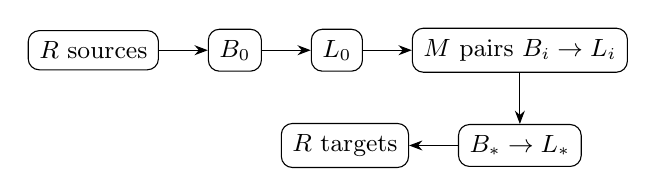
\begin{tikzpicture}[>=Stealth,node distance=0.55cm and 0.62cm,
 every node/.style={font=\small},box/.style={draw,rounded corners,inner sep=4pt}]
\node[box](s){$R$ sources};
\node[box,right=of s](b0){$B_0$};
\node[box,right=of b0](l0){$L_0$};
\node[box,right=of l0](bi){$M$ pairs $B_i\to L_i$};
\node[box,below=0.65cm of bi](bst){$B_\ast\to L_\ast$};
\node[box,left=of bst](t){$R$ targets};
\draw[->](s)--(b0);\draw[->](b0)--(l0);\draw[->](l0)--(bi);
\draw[->](bi)--(bst);\draw[->](bst)--(t);
\end{tikzpicture}
\end{center}
Every source--target entry is the sum of $M$ unit path products. Thus for
odd $M$ the transferred matrix is the all-ones $R\times R$ matrix, with
rank one. The closed critical homology dimension is $2R-2$.

\begin{proposition}[Internal-cut separation]\label{prop:separation}
For odd $M$, this graph has
\[
 |V|=2R+2M+4,\qquad |E|=2R+3M+2.
\]
The endpoint reference evaluates $R(3M+R+3)$ coefficient edges in either
forward or reverse direction. First-hit factorization at $\{B_0\}$ uses
$3M+2R+2=|E|$ coefficient compositions and produces a rank-one factorization.
Its minimum cut has capacity one. Taking even $R$ and $M=R^2+1$ gives
$\Theta(R^3)$ endpoint propagation work versus $O(R^2\log(R+2))$ total
index-word work for cut discovery, factor construction, and rank, with
$O(R^2)$ stored graph words. The terminal budget rejects without evaluating
the factors for every $R\geq2$.
\end{proposition}
\begin{proof}
The vertex and edge counts follow by listing the $2R$ critical vertices,
$2(M+2)$ matched vertices, $2R+2M$ nonmatching edges, and $M+2$ reversed
identity edges. For a fixed source, forward propagation traverses its first
edge, the next identity, the $M$ outward nonmatching arrows, the $M$ reversed
identities, the $M$ inward nonmatching arrows, the final identity, and the $R$
output arrows. Since $M$ is odd, the value at $B_\ast$ is nonzero. The
count is $3M+R+3$. Symmetry gives the same reverse count per target.

The first-hit prefix at $B_0$ traverses $R$ edges. Its unrestricted suffix
traverses $1+M+M+M+1+R$ edges. The total is $3M+2R+2$.
The one-dimensional vertex $B_0$ separates all paths. At least one path
exists, so a unit integral flow certifies minimum capacity one.
Edmonds--Karp performs one augmentation and a final unsuccessful search on
this family. Topological sorting and indexed representation therefore
cost $O((R+M)\log(R+M+2))$ word operations; factor evaluation is linear in
the graph size. Rank of the one-column/one-row factorization costs $O(R)$.
For $M=R^2+1$ these bounds give the claimed separation. Finally $S=2R$ and
$M(c,\kappa)=1$, so $\cutlb=2R-2>1$ for $R\geq2$.
\end{proof}

This is an exact asymptotic separation between specific complete rank-stage
implementations on valid algebraic complexes. It is not a new lower bound
for every algorithm computing their rank. Sparse Gaussian cancellation can
also exploit the shared structure efficiently. No realization of this
family by classical knot prefixes is proved, and its even total homology
dimension makes a direct reduced-knot interpretation particularly
inappropriate. The role of the family is to expose and test the internal
sharing that both endpoint choices repeat.

\section{Implementation, certificates, and executed validation}
\subsection{Module boundaries}
The package uses only Python's standard library. \code{core.py} implements
typed DAG validation, three coefficient adapters, endpoint propagation,
first-hit factors, factorized binary rank, weighted minimum cuts, and an
independent cut/flow verifier. \code{budgets.py} implements
Theorem~\ref{thm:budget}. \code{closure.py} checks marked matching dimensions,
not cobordism maps. \code{decision.py} implements the actual cut-only
preflight and exact fallback.

\code{cube.py} constructs a small reduced binary Khovanov cube for a closed
braid, validates grading and $d^2=0$, constructs a deterministic partial
acyclic matching, and exports the resulting scalar transfer graphs.
It is intentionally exponential and rejects input beyond eleven crossings.
Its matching-edge limit bounds the number of candidate edges considered;
it is not the number of matched pairs. No claim about optimal matchings is
made. The experiment uses limits 12 and unbounded on each small diagram.

The topological coefficient conventions are written out in Appendix A.
They provide a checkable bridge to real knots, rather than merely declaring
random graded matrices to be knot data. Still, this small cube constructor
is not an independent established knot-software oracle. The test suite
also checks known examples and elementary braid transformations to exercise
that bridge.

\subsection{Portable braid certificates and verifier independence}
\code{certificates.py} produces certificates containing the input braid,
a deterministic hash of its reconstructed cube, the matching pairs,
per-degree cut vertices and feasible flows, transferred ranks, and the final
reduced rank and verdict. The verifier reconstructs the cube, checks the
matching and graph acyclicity, verifies each cut/flow pair, and recomputes
transferred ranks by \emph{dense endpoint propagation}. It does not call
the matching search, minimum-cut optimizer, first-hit factorizer, or
factorized-rank routine.

This is useful implementation independence, not independence from all
mathematical assumptions. Producer and verifier share the cube constructor,
coefficient conventions, and generic binary-rank primitive. The verifier
is not polynomial in the original crossing count, and the certificate
format is not offered as a new complexity-class certificate. Hashes bind
files and reconstructed inputs; they do not prove topology.

Six braid certificates are supplied and were replayed successfully.
Mutation tests alter rank, input word, matching, or cut capacity and require
rejection. A separate mocked test makes factor evaluation raise an exception
and confirms that a cut-only rejection does not call it. Another test has
lower bound one and exact rank three, guarding against unsound early
acceptance.

\subsection{Unit tests and cross-checks}
The executed unit-test command is
\begin{lstlisting}
PYTHONPATH=code python -m unittest discover -s tests -v
\end{lstlisting}
It passed 36 tests. These test methods contain multiple exhaustive or seeded
subcases: valid separators in random small DAGs, all weighted cuts in small
graphs, 500 brute-force budget comparisons, and 40 additional random knot
closures, among others. They are not counted as separate unit tests.

The categorical comparisons cover $\F$, the square-zero dot algebra, and
typed rectangular matrices. They include non-antichain cuts, cut terminals,
empty separators when no terminal path exists, cancelled path sums,
nilpotent products, and noncommuting compositions. Weighted-cut tests include
zero and thousand-bit capacities. Graded budget tests include missing degree
intervals and dimensions whose labels must not be expanded. The cube tests
include mirrors, cancelling inverse generators, the three-strand braid
relation, and positive and negative Markov stabilization on small examples.
These finite tests support the implementation; the general correctness
claims rest on the proofs, not on statistical extrapolation.

\subsection{An 80-diagram knot-complex audit}
The seeded corpus consists of eight named or elementary braid examples and
72 random one-component braid closures. Random diagrams use two to four
strands and two to seven crossings; words are retained verbatim in the data.
The same knot may occur repeatedly under different diagrams. No claim of
80 distinct knot types or of an adversarial hard-knot corpus is intended.

For every diagram we construct the full reference cube and its independently
eliminated bigraded homology, then compare two Morse configurations.
The result is 160 configurations and 1,070 transferred maps, with no
entrywise transfer, factor-rank, or bigraded homology disagreement.
Across the 80 original cubes there are 24,556 allocated generators.

Twenty-four diagrams have reduced rank greater than one. All 24 are rejected
by cut-only preflight in both matching configurations, giving 48 rejections
without transferred-map evaluation. This does not mean that their prior
cube construction was avoided. The sharp bound strictly exceeds the naive
global capacity bound in 52 configurations and strictly exceeds the sum of
local nonnegative bounds in 51. These are finite-corpus observations, not a
general detection-completeness theorem for preflight.

\begin{center}
\small
\begin{tabular}{lrrrr}
\toprule
Named diagram & Crossings & Cube generators & Reduced rank & Full-match critical\\
\midrule
Crossingless unknot & 0 & 1 & 1 & 1\\
Positive RI unknot & 1 & 3 & 1 & 1\\
Negative RI unknot & 1 & 3 & 1 & 1\\
Trefoil & 3 & 15 & 3 & 3\\
Figure-eight & 4 & 33 & 5 & 5\\
$T(2,5)$ & 5 & 123 & 5 & 5\\
Stabilized unknot & 2 & 9 & 1 & 1\\
Cancelled-generator unknot & 3 & 15 & 1 & 1\\
\bottomrule
\end{tabular}
\end{center}

\section{Measurements: speedups, overhead, and what was not timed}
\subsection{Paired protocol}
All arms answer the same \emph{exact differential-rank query} on the same
preconstructed graph or collection of degree graphs. The forward and reverse
arms construct the full endpoint transfer matrix and take its binary rank.
The cut-factor arm includes network construction, exact minimum-cut search,
cut/flow verification, first-hit factors, and binary rank through those
factors. The control arm is identical to forward.

Every arm is warmed once. Seven rounds then execute a seeded shuffled arm
order, with garbage collection before each timing and fresh algorithm-local
arrays in each call. Timings use \code{perf\_counter\_ns}; medians are
reported. These short local timings are not hardware-independent constants.
The raw round order, individual values, Python version, platform, corpus,
and counts are retained in \code{results/}.

Graph construction, cube construction, and Morse matching are excluded from
\emph{every} timed arm. No production \code{fastunknot} scanner, minimum-fill
sparse reducer, recognition filter, ordering heuristic, or Rust port is
benchmarked. The cut-only decision shortcut is validated separately, not
substituted for exact rank in the timing comparison.

\subsection{Small actual knot complexes: discovery overhead dominates}
The following medians are milliseconds for all transfer maps of the named
partial-matching configuration. Values below one millisecond should be
interpreted with the accompanying A/A control, not as precise universal
ratios.
\begin{center}\begin{tabular}{lrrrrr}\toprule
Case & Forward & A/A control & Reverse & Cut-factor & F/C\\\midrule
trefoil & 0.054 & 0.056 & 0.055 & 0.130 & 0.41\\
figure\_eight & 0.125 & 0.127 & 0.129 & 0.455 & 0.27\\
torus\_2\_5 & 0.497 & 0.480 & 0.478 & 2.130 & 0.23\\
\bottomrule\end{tabular}\end{center}

The cut-factor method is slower by approximately $2.41\times$, $3.64\times$,
and $4.29\times$ respectively against forward propagation. The graphs and
endpoint sets are too small for internal sharing to repay network and
verification overhead. This is evidence against changing the default
reducer on the basis of this package, not a reason to conceal the measurements.

\subsection{Constructed bottleneck family: an increasing separation}
The next table records exact composition counts for
Proposition~\ref{prop:separation}. In every row the forward and reverse
counts coincide. The first-hit count equals the graph's edge count.
\begin{center}\begin{tabular}{rrrrrr}\toprule
$R$ & $M$ & Vertices & Edges & Endpoint compositions & First-hit compositions\\\midrule
8 & 65 & 150 & 213 & 1648 & 213\\
16 & 257 & 550 & 805 & 12640 & 805\\
32 & 1025 & 2118 & 3141 & 99520 & 3141\\
64 & 4097 & 8326 & 12421 & 790912 & 12421\\
\bottomrule\end{tabular}\end{center}

At $R=64$, first-hit propagation uses 12,421 compositions instead of
790,912, a count reduction of approximately $63.68\times$. This is not the
wall-clock speedup because both graph work and minimum-cut discovery are
included in the complete cut-factor arm.
\begin{center}\begin{tabular}{lrrrrr}\toprule
Case & Forward & A/A control & Reverse & Cut-factor & F/C\\\midrule
$R=8$ & 0.528 & 0.536 & 0.540 & 0.790 & 0.67\\
$R=16$ & 3.394 & 3.366 & 3.417 & 2.750 & 1.23\\
$R=32$ & 25.819 & 24.758 & 26.733 & 10.897 & 2.37\\
$R=64$ & 191.937 & 192.894 & 189.887 & 39.957 & 4.80\\
\bottomrule\end{tabular}\end{center}

At the smallest size discovery overhead still wins against factorization.
At the largest size the complete cut-factor rank stage is about
$4.80\times$ faster than forward propagation and $4.75\times$ faster than
reverse propagation. The A/A medians are also shown. These results support
the proved sharing mechanism on an algebraic stress family. They neither
establish a speedup on difficult classical knots nor compare against the
maintained sparse-cancellation default, which could exploit the same family
in a different way.

\subsection{Reproduction and interpretation}
Run the full driver with
\begin{lstlisting}
PYTHONPATH=code python code/run_experiments.py
\end{lstlisting}
It reconstructs the seeded corpus, verifies exact equalities, runs the paired
experiments, writes raw JSON and CSV, and regenerates the six example
certificates. Re-running it changes timing samples, not the expected exact
counts or homology comparisons. The numerical tables in this PDF are a
frozen rendering of the delivered run; the supplied table generator updates
them from a new result file. Time comparisons should be based on paired
results from one environment rather than copied between machines.

\section{Integration plan and safety of topological verdicts}
\subsection{An additive, opt-in integration boundary}
A suitable first integration is a research subdirectory under
\path{Topology/UnknotRecognition/reports/closure_cut_transfer/}, preserving
the maintained recognizer unchanged. No numeric report identifier is assumed
available. The independent code can be imported or run from that directory,
and the article can be linked from the synthesis overview after review.

A production implementation should first export a validated degree graph
from the existing graded/corridor transfer boundary and compare every
expanded first-hit map against the existing implementation. It should then
attach a verified fixed-closure adapter and compare graded closed matrices.
Only after these two bridges are established should the cut-only homology
budget be permitted to produce a recognition verdict.

It is especially important not to feed the new rank-only answer back into
an unfinished tangle scan. A rank does not encode the transferred morphism,
and the future continuation can distinguish maps of equal rank before
closure. Full typed factors can remain useful for further algebra only if
all subsequent operations are defined on that representation and preserve
its semantics. That is a separate implementation and proof task.

\subsection{Transactional and resource obligations}
The reference code rejects cyclic graphs, invalid cuts, malformed basic
encodings, mismatched types encountered in composition, and link inputs to
the knot-certificate wrapper. This is not a complete hostile-input or
resource-management layer. A real adapter must validate all coefficients
and endpoint types before trusting graph-derived data, account for actual
allocated arrays, poll cancellation/deadline limits during flow and algebra,
and preserve the previous valid state if installation fails.

A safe production policy builds a prospective replacement and its evidence
without mutating the live complex, verifies all dimensions and maps needed
for the selected branch, checks the remaining budget, and only then
commits an exact state or a certified verdict. Failure to finish becomes
\code{UNKNOWN} or an exact fallback on the preserved input. It is never
interpreted as knottedness, triviality, or a rank bound.

Cut search itself can be optional. A separator supplied by a crossing order,
a previously computed corridor, or an inexpensive heuristic can be verified
and used directly. Exact minimum-cut search is relevant when its stronger
cap repays its overhead. No competitive scheduling theorem for choosing
among sparse cancellation, endpoint propagation, and internal cuts is proved
here.

\subsection{Proof and engineering checklist before promotion}
The contract must bind a graph to a particular input knot, matching/scalar
contraction, boundary marking, grading convention, and fixed closure.
Certificate checks must establish acyclicity, scalar contraction validity,
closure dimensions, and coefficient types. For terminal acceptance, the
complete rank calculation must be covered; a narrow quantum or homological
window that merely agrees with the unknot is not sufficient. For rejection,
one certified lower bound above one is sufficient, but every assumption
supporting that lower bound must still be checked.

Finally, benchmarks intended to justify a default change must include the
full recognizer, existing filters, order selection, diagram preparation,
resource handling, and all proposed adapter costs. The present data isolate
one research boundary and intentionally stop short of that claim.

\section{Further research questions and proposed next results}
\subsection{Closure-aware separator profiles on genuine hard inputs}
For an actual verified transfer graph, measure the profile
\[
(h,j)\longmapsto (V_{h,j},E_{h,j},a_{h,j},b_{h,j},r_{h,j}^{\rm cut},\kappa_{h,j}).
\]
Here $r^{\rm cut}$ denotes cut cardinality, not differential rank. The first
experimental question is whether difficult classical knot diagrams ever
have small \emph{weighted} internal cuts that are not already handled well
by sparse elimination or endpoint-direction choice. A useful study should
include diagrams surviving the existing recognition filters, not merely a
random small braid corpus.

The proposed deliverable is an exact exporter plus frozen actual-stage
fixtures, with independent contraction and closure checks. A theorem about
one explicit infinite classical-knot family would be stronger evidence than
additional unrelated algebraic stress examples.

\subsection{Finding useful cuts without paying for exact flow}
Can a separator derived from the quantum order, a shared prefix, a shared
suffix, or a small number of articulation regions achieve capacity within a
provable factor of the minimum? A verified nonminimum cut is already sound.
The algorithmic objective should combine rank capacity, cut cardinality,
closure-evaluation cost, and expected propagation work; minimizing just one
of those quantities may choose an expensive representation.

A precise target is an approximation theorem for a weighted objective of
the form $\alpha\kappa+\gamma r+\sum_{q\in Q}\mathrm{evalcost}(q)$ on the
restricted DAGs arising from valid contractions. Any such theorem needs its
own proof: the ordinary unweighted path-budget greedy rule does not solve
this separator optimization.

\subsection{Basis-aware minimization of transfer interfaces}
Scalar basis changes alter $I,P,H$ and hence the corridor graph without
changing the represented homotopy type. Is there an efficiently certifiable
choice of scalar contraction that decreases a closure-capacity profile or
its sum? An unconstrained optimization over bases is too broad. One promising
restricted problem permits basis changes only inside fixed matching and
quantum blocks, with bounded-support representatives.

The desired result would state both the basis-search cost and the resulting
factor sparsity. A small cut obtained only after a dense exponential basis
change would not improve recognition complexity.

\subsection{Stronger numerical certificates using additional relations}
The budget theorem is sharp only given dimensions and separate rank caps.
Known zero maps, grading support, vanishing composites, symmetry, or shared
factor spaces can carry additional information. Can one incorporate such
information while retaining a polynomial-time certificate optimizer?
A carefully chosen extension might improve rejection without computing
ranks, but arbitrary matrix-rank constraints should not be assumed to reduce
to path matching.

A specific candidate is to record a common interface for several adjacent
maps together with a verified relation between their images and kernels.
The challenge is to formulate constraints stronger than
$x_{h-1}+x_h\leq c_h$ without guessing algebraic independence.

\subsection{Succinct multiplicities and the cost of knowing dimensions}
The dichotomy is most useful when $S$ can be computed before allocating all
$S$ basis vectors. Which maintained shared-component or twist representations
admit exact binary-encoded $c_{h,j}$ and a verifiable closure action on the
necessary maps? A useful theorem would prove polynomial-time extraction of
these counts in the compressed representation size and would bound the
factor dimensions required only in the unresolved branch.

The principal obstruction is that repeated objects can share dimensions
without sharing all incident morphisms. A representation must encode the
maps and their interactions, not simply replace equal matching labels by a
multiplicity counter.

\subsection{Persistence under crossing extension}
Can first-hit factors be updated after one crossing is appended without
expanding the old product? To obtain a general scanner improvement, one
needs formulas for extension, direct sums, delooping, and cancellation on
the factored representation, together with size bounds over many stages.
A small factorization at one terminal graph does not itself persist under
these operations.

A realistic intermediate theorem would treat a fixed number of prescribed
continuation types and establish bounded factor growth under that restricted
alphabet. A universal logarithmic-depth or quasi-polynomial-size statement
would require genuinely new geometric or categorical control.

\subsection{Decision-first certificates beyond rank one}
For any threshold $b$, the same proof gives the algebraic dichotomy
\[
\cutlb>b\quad\text{or}\quad S\leq2M+b.
\]
Can thresholded computations accelerate other link invariants or certified
homology queries after the topological meaning of the threshold is fixed?
This extension is algebraically immediate; its usefulness and appropriate
normalization for links are not. The one-component unknot contract must not
be silently reused for arbitrary link thresholds.

\subsection{Formal verification and certificate minimization}
The typed first-hit theorem, cut verification, and greedy rank-budget proof
are small enough to be plausible early formalization targets. A next artifact
could formalize finite-DAG path decomposition and the exchange proof in Lean,
then connect the statements to the existing matching or cobordism structures.
The present package contains no Lean files and claims no formal verification.

The example braid certificates deliberately use a dense independent verifier.
A useful engineering improvement would reduce verifier work while retaining
independence, for example by supplying checked basis and image certificates
for $\im A$ and $B(\im A)$. That would improve certificate replay, not
eliminate the need to bind the factors to a genuine knot complex.

\subsection{A class theorem with an affordable construction}
The most consequential missing result is an explicit class of difficult
classical diagrams for which the \emph{construction}, closure work, graph
sizes, and capacity budget in Corollary~\ref{cor:qpoly} are all bounded in
terms of the input size. Logarithmic boundary width alone is insufficient.
The theorem should identify a geometric condition that can itself be checked
or supplied with bounded-size evidence.

A successful class theorem would turn the current terminal algebra into an
end-to-end asymptotic improvement. Without that step, further refinement of
matrix evaluation alone does not establish the target for unrestricted knots.

\subsection{Relationship with hierarchy-based recognition}
A homological terminal certificate and a geometric hierarchy certificate can
be complementary exact branches in a recognizer. Any proposed portfolio
should retain independent provenance and costs for both branches. The new
cut theorem supplies no bound for constructing hierarchy surfaces, compressed
cutting, or the cost of essential-pattern tests. Conversely, a geometric
simplification that constructs a small verified terminal tangle might make
our capacity analysis useful. Finding such a precise interface is a research
question, not an equivalence asserted here.

\section{Conclusion and claim ledger}
The internal interface matters in two different ways. It can share a large
path sum more efficiently than either endpoint direction, and its closed
dimension can limit how much differential rank is available to remove
critical homology. The latter effect leads to the sharp budget theorem and
a rejection-or-small-terminal-dimension dichotomy. These are exact algebraic
statements, and the implementation exercises them both on genuine small
knot complexes and on a controlled algebraic separation family.

The main bottleneck that remains is not an algebraic identity left unchecked.
It is the construction and maintenance of an affordable, topologically
verified representation on arbitrary inputs. The numerical evidence also
argues for an optional research integration rather than a default replacement:
cut discovery loses on the small actual knot rank stages tested here.
\begin{center}
\begin{tabular}{p{0.56\linewidth}p{0.34\linewidth}}
\toprule
Claim & Status\\
\midrule
First-hit factorization for arbitrary typed DAG cuts & Proved; categorical tests passed\\
Closure-capacity rank upper bounds & Proved under a verified functor contract\\
Optimal budget and sharpness from dimensions/caps & Proved; exhaustive small comparisons passed\\
Rank-one rejection/dimension dichotomy & Proved for certified closed knot complexes\\
Independent small-braid certificate replay & Implemented; six supplied certificates verified\\
General production cobordism closure adapter & Not implemented in this package\\
Full maintained upstream test suite and recognizer benchmarks & Not run here\\
Quasi-polynomial algorithm for arbitrary input diagrams & Not established here\\
\bottomrule
\end{tabular}
\end{center}
The contribution is therefore a proof-supported research extension with
reproducible validation, explicit asymptotic scope, and concrete next theorem
targets, rather than an unverified claim of a general complexity breakthrough.

\appendix
\section{Reference reduced-cube conventions}
A braid word on $s$ strands is an integer list $w_1,\ldots,w_n$ with
$1\leq|w_i|<s$. The permutation obtained by swapping positions
$|w_i|,|w_i|+1$ at each generator determines the number of closure components.
The knot-certificate wrapper requires one cycle. For each crossing, positive
zero-resolution means vertical arcs and positive one-resolution means
cap--cup; the negative generator swaps those choices. Union--find computes
resolution circles after identifying the top and bottom of each strand.
The circle containing the first closure strand is marked.

The Frobenius algebra is $A=\F[x]/(x^2)$ with
\[
 m(1,1)=1,\quad m(1,x)=m(x,1)=x,\quad m(x,x)=0,
\]
\[
 \Delta(1)=1\otimes x+x\otimes1,\qquad\Delta(x)=x\otimes x.
\]
We use the marked subcomplex in which the marked circle always has label
$x$, and shift its reduced grading by $+1$. With state $\sigma$, let
$|\sigma|$ be its number of one-resolutions, $c(\sigma)$ its number of circles,
and $u$ the number of $x$ labels including the mark. The normalized bidegree is
\[
 h=|\sigma|-n_-,\qquad
 j=|\sigma|+n_+-2n_-+c(\sigma)-2u+1.
\]
A cube edge raises $h$ by one and preserves $j$. Binary coefficients avoid
cube signs. The code checks these statements for every constructed edge and
checks $d^2=0$ on every generator before using the complex.

The reference construction enumerates all $2^n$ resolutions and all reduced
circle labellings. Both memory and work can be exponential. The eleven-crossing
cap is an explicit safety limit on this research utility, not a theorem
that larger diagrams are difficult or that exhausting the cap has any
mathematical meaning.

\section{Algorithm summaries and certificate formats}
\subsection{First-hit transfer}
\begin{lstlisting}
check graph is a finite typed DAG
check Q separates all sources from all targets
for q in Q:
    A[q, :] = reverse_propagation_from(q,
                    stop_at_other_vertices_of_Q=True)
    zero A[q, s] for every s in Q with s != q
    B[:, q] = unrestricted_forward_propagation_from(q)
return (A, B)  # exact identity D = B*A
\end{lstlisting}
A stopped vertex may receive a value, but it must not propagate that value
or be included as another cut source's first-hit contribution. Identities
at cut terminals represent length-zero paths. These conventions account for
the terminal-cut regression cases.

\subsection{Decision preflight}
\begin{lstlisting}
verify input complex/contraction/closure contract
compute closed critical dimensions c[h,j]
for every adjacent-degree transfer graph:
    find or receive a vertex separator
    verify the separator and its closure-weighted capacity
compute M = maximum compatible sum of ranks by the greedy rule
lower = sum(c) - 2*M
if lower > 1:
    return certified rank-not-one  # knot rejection only with origin contract
otherwise:
    compute exact transferred ranks through first-hit factors
    beta = sum(c) - 2*sum(exact_ranks)
    return exact beta
\end{lstlisting}
The prototype uses unit capacities on already evaluated scalar graphs.
The theorem also covers weighted typed graphs once a verified closure
adapter provides their dimensions and maps.

\subsection{Cut certificate}
A cut certificate stores the cut-vertex list, its capacity, and one flow
integer per arc of a canonical node-split network. Verification checks:
nonnegative capacities and flows; every flow within its capacity; conservation
at all nonterminal network vertices; the asserted total value; and absence
of a surviving source--target path after deleting the cut. Equality of flow
value and cut capacity proves optimality. For a nonminimum but valid rank
cap, only the separation and dimension checks are necessary.

\subsection{Braid-certificate commands}
From the package root:
\begin{lstlisting}
PYTHONPATH=code python -m separator_transfer braid \
  --strands 3 --word '[1,-2,1,-2]' \
  --certificate examples/my_figure_eight.json
PYTHONPATH=code python -m separator_transfer verify \
  examples/my_figure_eight.json
\end{lstlisting}
These commands are reference computations on a small diagram. They do not
call the maintained production recognizer. User-supplied files can be
modified arbitrarily, so a verifier must rebuild and check the required
mathematical data rather than trusting the verdict field.

\section{Artifact map and reproducibility scope}
\begin{center}
\begin{tabular}{p{0.39\linewidth}p{0.51\linewidth}}
\toprule
Path & Purpose\\
\midrule
\code{article/article.tex}, \code{references.bib} & Complete article and primary references\\
\code{article/article.pdf} & Compiled and visually inspected report\\
\code{code/separator\_transfer/} & Exact transfer, flow, budget, cube, and certificate modules\\
\code{code/run\_experiments.py} & Seeded audit and paired benchmark driver\\
\code{tests/test\_research.py} & 36 unit tests with exhaustive and seeded subcases\\
\code{results/knot\_audit.json} & Every diagram, matching configuration, and exact result\\
\code{results/benchmarks.json} & Raw paired samples and measurement scope\\
\code{results/summary.json} & Auditable summary counts and medians\\
\code{examples/} & Six independently replayed braid certificates\\
\code{PROVENANCE.json}, \code{INTEGRATION.md} & Reviewed-source identifiers and adapter obligations\\
\code{SHA256SUMS} & Hashes of delivered files other than the manifest itself\\
\bottomrule
\end{tabular}
\end{center}
The package includes no font files, third-party paper PDFs, or copied
production source. It is intended to be reviewed and integrated as an
additive research artifact. Exact results are deterministic under the stated
encoding and seed; timing values are observations from the delivered run.

\bibliographystyle{plainnat}
\bibliography{references}
\end{document}
